\section*{ÔN TẬP KIỂM TRA CUỐI KÌ 2 - ĐỀ 03}
\setcounter{ex}{0}\setcounter{bt}{0}
\Opensolutionfile{ans}[ans/ansBTTeX1]

\noindent\textbf{I. PHẦN TRẮC NGHIỆM:}
%Câu 1
\begin{ex}
Với $a,b>0$, $\alpha ,\beta $ là các số thực bất kì, đẳng thức nào sau đây sai?
\choice
{$\dfrac{a^{\alpha}}{b^{\beta}}=\left(\dfrac{a}{b}\right)^{\alpha -\beta }$}
{${a^{\alpha }} \cdot {a^{\beta }}={a^{\alpha +\beta }}$}
{${a^{\alpha }} \cdot {b^{\alpha }}={{(ab)}^{\alpha }}$}
{$\dfrac{{a^{\alpha }}}{{a^{\beta }}}={a^{\alpha -\beta }}$}
\end{ex}
%Câu 2
\begin{ex}
Trong các hàm số sau, hàm số nào là hàm số mũ ?
\choice
{$y=\log x$}
{$y=\dfrac{x^2}{3}$}
{$y={{10}^x}$}
{$y=\dfrac{3}{\log _2x}$}
\end{ex}
%Câu 3
\begin{ex}
Trong các hàm số sau, hàm số nào là hàm số lôgarit?
\choice
{$y=\log _5x$}
{$y=\dfrac{\log _25}{x}$}
{$y=\left(\sqrt{2}\right)^x$}
{$y=\dfrac{x^2}{\ln 3}$}
\end{ex}
%Câu 4
\begin{ex}
\immini{
Cho $a,b,c$ là các số thực dương khác $1$. Đồ thị của ba hàm số $y=a^x,y=b^x,y=c^x$ như hình vẽ.
Khẳng định nào sau đây là đúng?
\choice
{$b>1$}
{$0<c<1$}
{$0<a<b<1<c$}
{$0<b<a<1<c$}
}{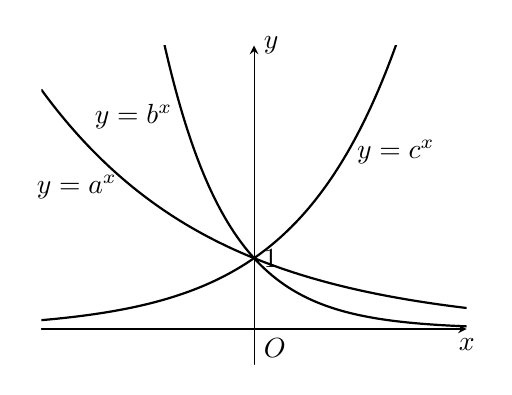
\begin{tikzpicture}[line join = round, line cap = round, >=stealth, scale = .9]
%Hệ trục Oxy và hàm số cần vẽ
\def\xmin{-3}     \def\xmax{3}
\def\ymin{-.5}       \def\ymax{4}
\def\f(#1){(1/3)^(#1)}
\def\g(#1){(2/3)^(#1)}
\def\h(#1){2^(#1)}
%Vẽ hệ trục
\draw[->] (\xmin,0)--(0,0) node[below right]{$O$}--(\xmax,0) node[below]{$x$};
\draw[->] (0,\ymin)--(0,\ymax) node[right]{$y$};
\draw (0,1)node[right]{$1$} (-2.5,2)node{$y=a^x$} (-1.7,3)node{$y=b^x$} (2,2.5)node{$y=c^x$};
%Vẽ hàm số
\begin{scope}
\clip (\xmin,\ymin) rectangle (\xmax,\ymax);
\draw[smooth, thick, black] plot[domain = \xmin:\xmax, samples = 200, variable=\x]({\x},{\f(\x)});
\draw[smooth, thick, black] plot[domain = \xmin:\xmax, samples = 200, variable=\x]({\x},{\g(\x)});
\draw[smooth, thick, black] plot[domain = \xmin:\xmax, samples = 200, variable=\x]({\x},{\h(\x)});
\end{scope}
\end{tikzpicture}
}
\end{ex}
%Câu 5
\begin{ex}
Nghiệm của phương trình $\log _3(5x)=2$ là
\choice
{$x=\dfrac{8}{5}$}
{$x=9$}
{$x=8$}
{$x=\dfrac{9}{5}$}
\end{ex}
%Câu 6
\begin{ex}
Nghiệm của phương trình ${3^{x-1}}=9$ là
\choice
{$x=-2$}
{$x=2$}
{$x=-3$}
{$x=3$}
\end{ex}
%Câu 7
\begin{ex}
Tập nghiệm của bất phương trình $\log x\ge 1$ là
\choice
{$\left(10;+\infty\right)$}
{$\left(0;+\infty\right)$}
{$\left(-\infty ;10\right)$}
{$\left[10;+\infty\right)$}
\end{ex}
%Câu 8
\begin{ex}
Giới hạn (nếu tồn tại) nào sau đây dùng để định nghĩa đạo hàm của hàm số $y=f(x)$ tại$x_0$?
\choice
{$ \lim\limits_{h\to 0} \,\dfrac{f(x+h)-f(x_0)}{h}$}
{$ \lim\limits_{x\to 0} \,\dfrac{f(x)-f(x_0)}{x-x_0}$}
{$ \lim\limits_{x\to x_0} \,\dfrac{f(x)-f(x_0)}{x-x_0}$}
{$ \lim\limits_{h\to 0} \,\dfrac{f(x_0+h)-f(x)}{h}$}
\end{ex}
%Câu 9
\begin{ex}
Cho hàm số $y=-x^2+1$ có đồ thị $(C)$. Viết phương trình tiếp tuyến của đồ thị $(C)$ tại điểm có hoành độ bằng $2$.
\choice
{$y=-4x+5$}
{$y=-4x+13$}
{$y=-4x-13$}
{$y=4x-5$}
\end{ex}
%Câu 10
\begin{ex}
Khẳng định nào sau đây sai?
\choice
{$(2024^x)'=2024^x \ln 2024$}
{$(\ln x)'=\dfrac{1}{x}$}
{$(x^2-3x+1)'=2x-3$}
{$(e^{2x})'={e^{2x}}$}
\end{ex}
%Câu 11
\begin{ex}
Đạo hàm của hàm số $y=2024-\cos 2x$ là
\choice
{$y'=2024-\sin 2x$}
{$y'=2024+2\sin x$}
{$y'=-2\sin 2x$}
{$y'=2\sin 2x$}
\end{ex}
%Câu 12
\begin{ex}
Đạo hàm của hàm số $y=\dfrac{x+1}{2x-3}$ là
\choice
{$y'=\dfrac{-5}{(2x-3)^2}$}
{$y'=\dfrac{1}{(2x-3)^2}$}
{$y'=\dfrac{1}{2x-3}$}
{$y'=\dfrac{-5}{2x-3}$}
\end{ex}
%Câu 13
\begin{ex}
Cho hàm số $y=x^4-2x^2+\sqrt{x}-2$. Tính $y'(1)$.
\choice
{$y'(1)=\dfrac{1}{2}$}
{$y'(1)=\dfrac{1}{4}$}
{$y'(1)=-\dfrac{3}{2}$}
{$y'(1)=2$}
\end{ex}
%Câu 14
\begin{ex}
Cho hàm số $f(x)=\sin 2x-x$. Nghiệm của phương trình $f'(x)=0$ là
\choice
{$x=\pm \dfrac{\pi }{3}+k2\pi (k\in \mathbb{Z})$}
{$x=\pm \dfrac{\pi }{6}+k\pi (k\in \mathbb{Z})$}
{$x=\pm \dfrac{\pi }{6}+k2\pi (k\in \mathbb{Z})$}
{ $x=\pm \dfrac{\pi }{3}+k\pi (k\in \mathbb{Z})$}
\end{ex}
%Câu 15
\begin{ex}
Cho hàm số $f(x)=\log _5(x^2+2x+2)$. Tập nghiệm của bất phương trình $f'(x)>0$ là
\choice
{$S=\left(-2;+\infty\right)$}
{$S=\left(0;+\infty\right)$}
{$S=\left(1;+\infty\right)$}
{ $S=\left(-1;+\infty\right)$}
\end{ex}
%Câu 16
\begin{ex}
Cho hàm số $y=x^5-3x^4+x+1$. Tìm đạo hàm cấp hai của hàm số tại điểm $x$ bất kì?
\choice
{$y''=5x^3-12x^2+1$}
{$y''=5x^4-12x^3$}
{$y''=20x^2-36x^3$}
{$y''=20x^3-36x^2$}
\end{ex}
%Câu 17
\begin{ex}
Cho ${f(x)=x^3}$. Tính $f''(1)$.
\choice
{$f''(1)=3$}
{$f''(1)=2$}
{$f''(1)=6$}
{$f''(1)=1$}
\end{ex}
%Câu 18
\begin{ex}
Đạo hàm cấp hai của hàm số $y=\sin 2x$ là
\choice
{$y''=-\sin 2x$}
{$y''=-4\sin x$}
{$y''=-4\sin 2x$}
{$y''=-2\sin 2x$}
\end{ex}
%Câu 19
\begin{ex}
Đạo hàm cấp hai của hàm số $y=\cos ^2 3x$ là
\choice
{$y''=-18\cos 6x$}
{$y''=18\cos 6x$}
{$y''=2\cos 6x$}
{$y''=-2\cos 6x$}
\end{ex}
%Câu 20
\begin{ex}
Cho hàm số $y=f(x)={{(x+2)}^4}$. Tính $f''(2)$.
\choice
{$f''(2)=108$}
{$f''(2)=192$}
{$f''(2)=96$}
{$f''(2)=81$}
\end{ex}
%Câu 21
\begin{ex}
Cho hình lập phương $ABCD.A'B'C'D'$. Đường thẳng nào sau đây vuông góc với đường thẳng $BC'$?
\choice
{$A'D$}
{$AC$}
{$BB'$}
{$AD'$}
\end{ex}
%Câu 22
\begin{ex}
Cho hình chóp $S.ABCD$ có đáy $ABCD$ là hình chữ nhật, $SA\perp (ABCD)$. Mệnh đề nào sau đây đúng ?
\choice
{$BA\perp (SAD)$}
{$BA\perp (SAC)$}
{$BA\perp (SBC)$}
{$BA\perp (SCD)$}
\end{ex}
%Câu 23
\begin{ex}
Cho hình chóp $S.ABCD$ có đáy $ABCD$ là hình vuông và $SA\perp (ABCD)$. Gọi $M$ là hình chiếu vuông góc của $A$ lên cạnh $SB$. Khẳng định nào sau đây là đúng?
\choice
{$AM\perp SD$}
{$AM\perp (SCD)$}
{$AM\perp CD$}
{$AM\perp (SBC)$}
\end{ex}
%Câu 24
\begin{ex}
Cho hình chóp $S \cdot ABC$ có cạnh bên $SA$ vuông góc mặt đáy $(ABC)$. Góc tạo bởi $SB$ và đáy tương ứng là
\choice
{$\widehat{SCA}$}
{$\widehat{SBA}$}
{$\widehat{SBC}$}
{$\widehat{SAB}$}
\end{ex}
%Câu 25
\begin{ex}
Cho hình chóp tứ giác đều $S.ABCD$. Phát biểu nào sau đây đúng?
\choice
{Số đo của góc nhị diện $\left[S, AB, C\right]$ bằng $\widehat{SBC}$}
{Số đo của góc nhị diện $\left[D, SA, B\right]$ bằng ${{90}^{\circ }}$}
{Số đo của góc nhị diện $\left[S, AC, B\right]$ bằng ${{90}^{\circ }}$}
{Số đo của góc nhị diện $\left[D, SA, B\right]$ bằng $\widehat{BSD}$}
\end{ex}
%Câu 26
\begin{ex}
Cho hình chóp $S \cdot ABCD$ có đáy $ABCD$ là hình vuông cạnh $a$ và $SA\perp (ABCD)$. Biết rằng $SA=\dfrac{a\sqrt{6}}{3}$. Tính góc giữa $SC$ và $(ABCD)$.
\choice
{$30^\circ $}
{$65^\circ $}
{$75^\circ $}
{$45^\circ $}
\end{ex}
%Câu 27
\begin{ex}
Trong các mệnh đề, mệnh đề nào đúng?
\choice
{Hai mặt phẳng phân biệt cùng vuông góc với một mặt phẳng thì song song với nhau}
{Qua một đường thẳng có duy nhất một mặt phẳng vuông góc với một đường thẳng cho trước}
{Hai mặt phẳng phân biệt cùng vuông góc với một đường thẳng thì song song với nhau}
{Qua một điểm có duy nhất một mặt phẳng vuông góc với một mặt phẳng cho trước}
\end{ex}
%Câu 28
\begin{ex}
Cho hình chóp $S \cdot ABCD$ có đáy $ABCD$ là hình thoi, $SA=SC$. Khẳng định nào sau đây đúng?
\choice
{Mặt phẳng $(SBD)$ vuông góc với mặt phẳng $(ABCD)$}
{Mặt phẳng $(SBC)$ vuông góc với mặt phẳng $(ABCD)$}
{Mặt phẳng $(SAD)$ vuông góc với mặt phẳng $(ABCD)$}
{Mặt phẳng $(SAB)$ vuông góc với mặt phẳng $(ABCD)$}
\end{ex}
%Câu 29
\begin{ex}
Cho hình chóp $S \cdot ABC$ có đáy $ABC$ là tam giác vuông cân tại $B$, $SA$ vuông góc với đáy. Gọi $M$ là trung điểm $AC$. Khẳng định nào sau đây sai?
\choice
{$BM\perp AC$}
{$(SBM)\perp (SAC)$}
{$(SAB)\perp (SBC)$}
{$(SAB)\perp (SAC)$}
\end{ex}
%Câu 30
\begin{ex}
Cho hình lập phương $ABCD.A'B'C'D'$. Tính góc giữa mặt phẳng $(ABCD)$ và $\left(ACC'A'\right)$.
\choice
{${{45}^{\circ }}$}
{${{60}^{\circ }}$}
{${{30}^{\circ }}$}
{${{90}^{\circ }}$}
\end{ex}
%Câu 31
\begin{ex}
Cho hình chóp $S.ABCD$. có đáy là hình vuông cạnh $a$. Đường thẳng $SA$ vuông góc với mặt phẳng đáy, $SA = a$. Gọi $M$ là trung điểm của $CD$. Khoảng cách từ $M$ đến $(SAC)$ nhận giá trị nào trong các giá trị sau?
\choice
{$\dfrac{a\sqrt{2}}{2}$}
{$2a$ }
{$a\sqrt{2}$ }
{$a$ }
\end{ex}
%Câu 32
\begin{ex}
Cho hình lập phương $ABCD. A'B'C'D'$ có cạnh bằng $1$. Khoảng cách giữa $AA'$ và $BD'$ bằng
\choice
{$\dfrac{\sqrt{3}}{3}$}
{$\dfrac{\sqrt{2}}{2}$}
{$\dfrac{2\sqrt{2}}{5}$}
{$\dfrac{3\sqrt{5}}{7}$}
\end{ex}
%Câu 33
\begin{ex}
Hình chóp đều $S.ABC$ có cạnh đáy bằng $3a$ cạnh bên bằng $2a$. Khoảng cách từ $S$ đến $(ABC)$ bằng
\choice
{$2a$}
{$a\sqrt{3}$}
{$a$}
{$a\sqrt{5}$}
\end{ex}
%Câu 34
\begin{ex}
Cho hình chóp $S.ABCD$ có $SA\perp (ABCD)$, $SA=2a$, $ABCD$ là hình vuông cạnh bằng $a$, tâm $O$. Tính khoảng cách từ $O$ đến đường thẳng $SC$.
\choice
{$\dfrac{a\sqrt{3}}{3}$}
{$\dfrac{a\sqrt{3}}{4}$}
{$\dfrac{a\sqrt{2}}{3}$}
{$\dfrac{a\sqrt{2}}{4}$}
\end{ex}
%Câu 35
\begin{ex}
Tính thể tích $V$ của khối lập phương $ABCD.A'B'C'D'$, biết $AC'=a\sqrt{3}$.
\choice
{$V=\dfrac{2a^3}{9}$}
{$V=\dfrac{a^3}{3}$}
{$V=\dfrac{3a^3}{8}$}
{$V=a^3$}
\end{ex}

\noindent\textbf{II. PHẦN TỰ LUẬN}
%Câu 36 
\begin{ex} 
Giải phương trình $\log _3\left(x^2+4x\right)+\log_{\tfrac{1}{3}}(2x+3)=0$.
\end{ex}
%Câu 37
\begin{ex}
Viết phương trình tiếp tuyến đồ thị hàm số $y=2x^2-3x+1$ tại giao điểm với trục hoành.
\end{ex}
%Câu 38
\begin{ex}
Ba cầu thủ sút phạt đền $11m$ mỗi người đá một lần với xác suất làm bàn tương ứng là $x,y$ và $0,6$ với $x>y$. Biết rằng xác suất để ít nhất một trong ba cầu thủ ghi bàn là $0,976$ và xác suất để cả ba cầu thủ đều ghi bàn là $0,336$. Tính xác suất để có đúng hai cầu thủ ghi bàn. 
\end{ex}
%Câu 39
\begin{ex}
Cho tứ diện $ABCD$ có $\widehat{DAB}=\widehat{CBD}=90^\circ$, $AB=a$, $AC=a\sqrt{5};$ $\widehat{ABC}=135^\circ$. Biết số đo của góc nhị diện $\left[A, BD, C\right]$ là $150^\circ $. Tính thể tích của tứ diện $ABCD$
\end{ex}
\Closesolutionfile{ans}